\chapter{Implementation}\label{ch:implementation}

\section{Preparation}\label{sec:preparation2}

\subsection{Selection of blockchain network}\label{subsec:selection-of-blockchain-network}

As seen in \cref{tab:selection-of-blockchain-network}, the findings in~\cref{sec:voting-systems} can be applied as selection criteria for relevant \gls{Blockchain} networks (see \cref{subsec:comparison-of-turing-complete-blockchains}).
However, some properties mentioned in~\cref{sec:voting-systems} depend entirely on decisions relating to frontend design and code governance rather than the selected \gls{Blockchain}, e.g., whether the software is open-source.
These are displayed in gray in~\cref{tab:selection-of-blockchain-network}.

\begin{table}[H]
    \begin{tabularx}{\textwidth}{bCCCC}
        \hline
        \textbf{Property} & \textbf{Ethereum} & \textbf{Hyperledger Fabric} & \textbf{Polygon} & \textbf{Solana} \\
        \hline
        Auditability & \dblcmark & \dblcmark & \dblcmark & \dblcmark \\
        \hline
        Anonymity & \dblcmark & \cmark & \dblcmark & \cmark  \\
        \hline
        \rowcolor{lightgray}
        Usability & - & - & - & -  \\
        \hline
        \rowcolor{lightgray}
        Accessibility & - & - & - & - \\
        \hline
        Security & \dblcmark & \cmark & \dblcmark & \cmark   \\
        \hline
        Scalability & \xmark & \cmark & \cmark & \cmark  \\
        \hline
        \rowcolor{lightgray}
        Transparency & - & - & - & - \\
        \hline
        Incoercibility & \xmark & \xmark & \xmark & \xmark  \\
        \hline
    \end{tabularx}
    \caption{Comparison of blockchains based on voting system requirements}
    \label{tab:selection-of-blockchain-network}
\end{table}

All four \gls{Blockchain} networks possess most of the necessary properties.
Nevertheless, as shown in \cref{subsec:comparison-of-turing-complete-blockchains}, scalability seems to be a major issue underlying \gls{Blockchain} technology in general.
For instance, even though the Ethereum Foundation is looking to improve Ethereum's protocol further, theoretically enabling it to process up to 100,000 \gls{TPS} in the future, as of the time of this writing, it is not able to process enough transactions to facilitate national elections.
Conversely, other \glspl{Blockchain} compromise on similarly essential features to achieve a higher number of \gls{TPS}, e.g, security or network stability, the latter being an equally important scalability aspect.
Unfortunately, in the absence of a \gls{Blockchain} protocol that satisfies all aspects shown in~\cref{sec:voting-systems}, compromises in our selection process were unavoidable.
With this in mind and looking at \cref{tab:selection-of-blockchain-network}, Polygon seemed to be the most logical choice as it runs on top of Ethereum.
Therefore, it automatically benefits from Ethereum's superior security and anonymity, as well as all future improvements made to Ethereum's protocol, while still giving it an edge in terms of scalability due to its Layer 2 protocol (see~\cref{subsec:comparison-of-turing-complete-blockchains}).

\subsection{Selection of technology stack}\label{subsec:selection-of-tech-stack}

There are certainly many frameworks that could be used to develop the server- and client-side of a decentralized electronic voting system.
However, we relied on a full Node.js integration due to its non-blocking \gls{IO} to ensure high scalability (see~\cref{subsec:node.js}).
Similarly, given the scalability advantages of monorepos (see~\cref{subsec:nx}), we utilized nx to manage the project's repository.
Additionally, keeping transparency in mind (see~\cref{sec:voting-systems}), an open-source project built with nx is more accessible to other developers as a resource for future research.

We used Next.js as a framework on the client side as it allows for server-side rendering, increasing the application's overall security (see~\cref{subsec:next.js}) and making it \glstext{SEO}-friendly.
Alternatively, we could have developed the client-side with Nuxt.js, which mimics most of Next.js's server-side and static rendering methods while using Vue.js instead of React.js under the hood.
Nevertheless, Nuxt.js has a smaller community, arguably making React.js the preferable choice.

Although Next.js comes with its own routing framework for API calls, it is reasonable to use a separate framework for requests that handle database and smart contract actions.
Therefore, we utilized Nest.js, which eased the process of following best practices for developing backend applications.
As illustrated in~\cref{subsec:nest.js}, Nest.js is specifically designed with scalability in mind;
moreover, it ensures high readability for developers with either an \gls{OOP} or \gls{FP} background.
Likewise, we handled database-related aspects of the application using a PostgreSQL database since a broad spectrum of developers should be familiar with a \gls{ORDBMS} and PostgreSQL in particular (see~\cref{subsec:postgresql}).

\section{Setting up the workspace}\label{sec:setting-up-the-workspace}

\subsection{Creating a GitHub repository}\label{subsec:creating-a-git-repository}

\begin{figure}[h]
    \centering
    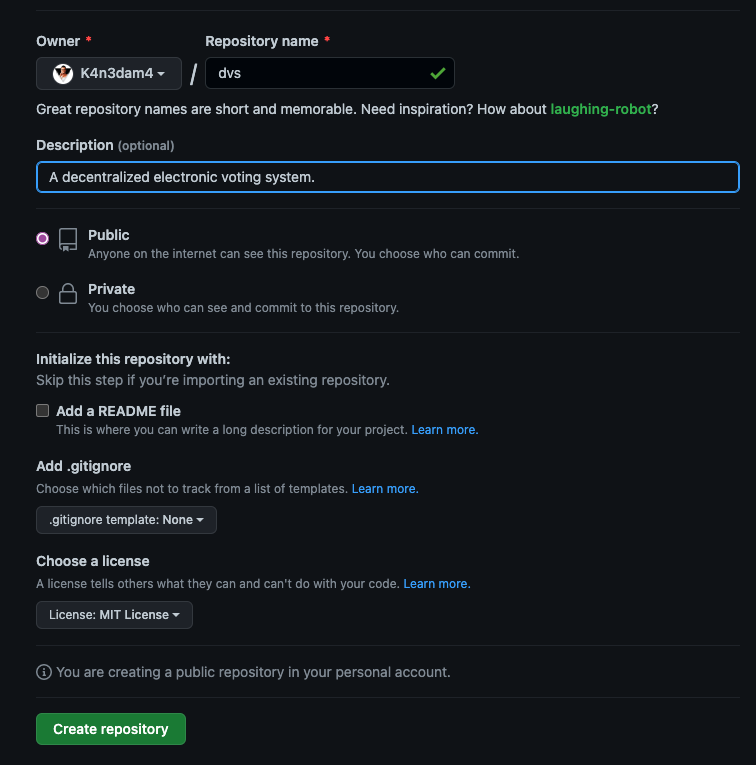
\includegraphics[scale=0.4]{initializing-repository}
    \caption{Creating a Github repository}
    \label{fig:initializing-repository}
\end{figure}

For the reasons discussed in~\cref{subsec:versioning}, the first step in the development process was the creation of a GitHub repository.
As seen in~\cref{fig:initializing-repository}, we changed the license from \emph{None} to \emph{MIT License}.
At the same time, the repository itself was initialized containing neither a README nor a .gitignore file, as these are automatically created by nx (see~\cref{subsec:creating-a-monorepo-using-nx}).

\subsection{Creating a monorepo using nx}\label{subsec:creating-a-monorepo-using-nx}

Creating a monorepo with nx is a straightforward process using the nx-provided executable package \emph{create-nx-workspace} with \gls{npx}.

\begin{figure}[h]
    \begin{subfigure}[b]{\textwidth}
        \centering
        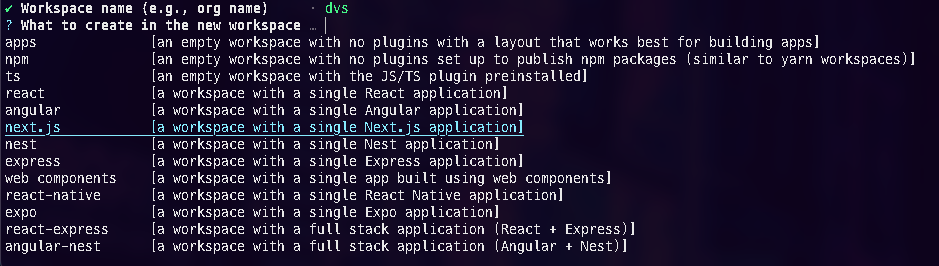
\includegraphics[width=\textwidth]{nx-workspace-options-0}
        \caption{Options for app templates nx can automatically build during initialization}
        \label{fig:nx-workspace-options-0}
    \end{subfigure}
    \begin{subfigure}[b]{0.5\textwidth}
        \centering
        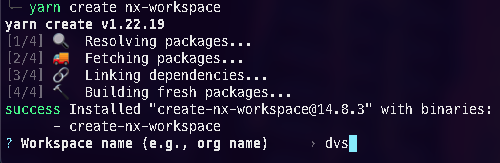
\includegraphics[width=\textwidth, height=85px]{nx-workspace-name}
        \caption{Naming the workspace}
        \label{fig:nx-workspace-name}
    \end{subfigure}
    \begin{subfigure}[b]{0.5\textwidth}
        \centering
        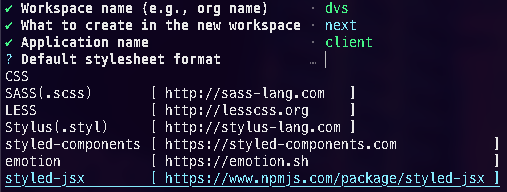
\includegraphics[width=\textwidth]{nx-workspace-options-1}
        \caption{Default style format options}
        \label{fig:nx-workspace-options-1}
    \end{subfigure}
    \caption{Setting up a nx workspace}
    \label{fig:setting-up-nx-workspace}
\end{figure}

After initiating the process by typing \mintinline{text}{yarn create nx-workspace} in the terminal, nx allows developers to name (see~\cref{fig:nx-workspace-name}) the project.
Next, developers are offered several template options for an initial application nx then automatically adds to the workspace (see~\cref{fig:nx-workspace-options-0,fig:nx-workspace-options-1}).
Given these options, we initialized the workspace with a Next.js application for the client side of the voting system.
Alternatively, we could have initialized it with Nest.js, but the order in which client and server applications were added to the workspace was irrelevant in this context.

\section{Setting up the backend}\label{sec:setting-up-a-nest.js-backend}

\subsection{Creating a Nest.js application}\label{subsec:creating-a-nest.js-application}

The installation of a plugin with \mintinline[breaklines]{text}{yarn add -D @nrwl/nest} was necessary to let nx handle the installation process of the Nest.js application.
After installing the plugin, we added a new Nest.js application to the workspace using the \mintinline[breaklines]{text}{nx g @nrwl/nest:app api} command, where \emph{api} is the name given to the application.

To maintain scalability, we combined Nest.js's modular design with nx's \emph{libs} directories, meaning backend controllers and services were split up and installed into \emph{libs/api} rather than the application directory.
As mentioned in~\cref{subsec:nx}, modularizing code within the \emph{libs} directory makes it reusable in all workspace applications sharing the same scope.
Hence, all future applications that might be added to the project will also be able to access that code if needed, thus making it easier to adhere to \gls{DRY} principles.

\subsection{Creating a PostgreSQL database}\label{subsec:creating-a-postgresql-database}

To handle database entries, we created a new Nest.js module, \emph{prisma}, in the \emph{libs/api} folder.
Then, we installed Prisma as a devDependency with \mintinline[breaklines]{text}{yarn add -D prisma}, which provided basic tooling for databases, such as creating type-safe schemas, a built-in migration system, and a \gls{GUI} to display and edit database entries.
Following the installation process, we created a docker-compose.yml, enabling the application to run dockerized PostgreSQL databases during development, test, or production builds (see listing~\ref{lst:docker-compose.yml}).

\codeFromFile{yaml}{code_snippets/docker-compose.yml}{Docker-compose.yml used in the prisma module}{Docker-compose.yml used in the prisma module}{lst:docker-compose.yml}

Having created a docker-compose file, along with the commands necessary to run the database in the prisma module’s project.json and the project’s package.json, we added a core Nest.js module (see listing~\ref{lst:core-module}) that makes configurations such as the database \gls{URL} available throughout the Nest.js application.
Consequently, we could connect the Nest.js application to the database through the prisma service (see listing~\ref{lst:prisma-service}) using the \gls{URL} from the core module.

\codeFromFile{ts}{code_snippets/nest-core-module.ts}{Core module}{Core module}{lst:core-module}
\codeFromFile{ts}{code_snippets/nest-prisma-service.ts}{Prisma service}{Prisma service}{lst:prisma-service}

\section{Smart Contracts}\label{sec:smart-contracts}
















